
\begin{document}

%%% Titulní strana práce a další povinné informační strany

%%% Titulní strana práce

\pagestyle{empty}
\pagenumbering{gobble}
\hypersetup{pageanchor=false}

\begin{center}
\LARGE
\textbf{GYMNASIUM JANA KEPLERA}\\
{\large Parléřova 2/118, 169 00 Praha 6}

\vspace{\stretch{3}}


\includegraphics[width=.3\textwidth]{img/logo}

\vspace{\stretch{3}}

{\Huge\bfseries\NazevPrace}

\vspace{8mm}
\mdseries{Maturitní práce}

\vspace{\stretch{8}}
\large
\begin{tabular}{rl}
Autor: & \AutorPrace \\
\noalign{\vspace{2mm}}
Třída: & \Trida\\
\noalign{\vspace{2mm}}
Školní rok: & 2020/2021\\
\noalign{\vspace{2mm}}
Předmět: & Informatika \\
\noalign{\vspace{2mm}}
Vedoucí práce: & \Vedouci \\
\end{tabular}

\vspace{20mm}
Praha, \DatumOdevzdani
\end{center}


\openright

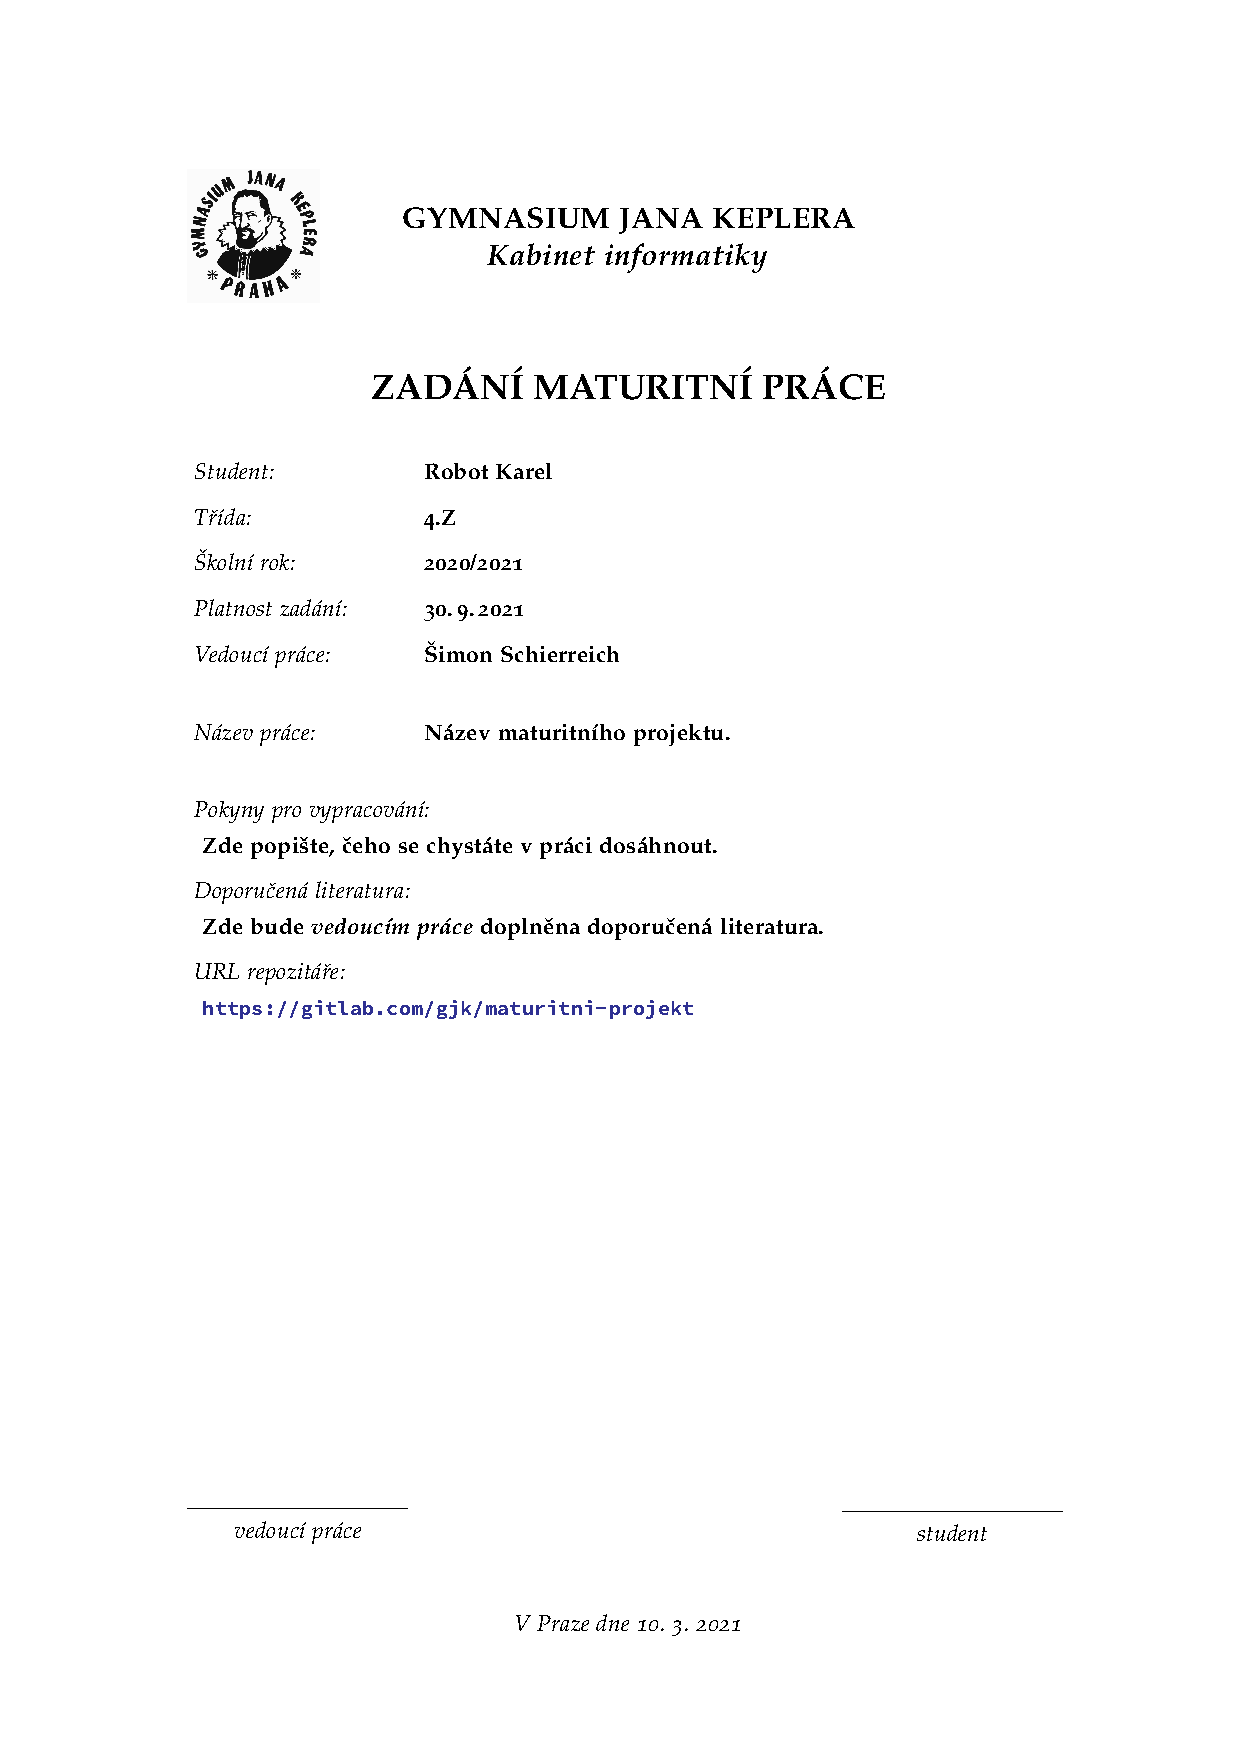
\includepdf[]{zadani.pdf}


%%% Strana s čestným prohlášením k bakalářské práci

\hypersetup{pageanchor=true}
\cleardoublepage
\vspace*{\fill}
\section*{Prohlášení}
\noindent
\Prohlaseni

\vspace{2cm}
\noindent
V Praze dne \today
\hspace*{\fill}\small{\AutorPrace}
\vspace{1cm}

%%% Poděkování
\openright
\vspace*{\fill}
\section*{Poděkování}
\noindent
\Podekovani
\vspace{1cm}


%%% Povinná informační strana bakalářské práce
\openright
\section*{Abstrakt}
\noindent
\Abstrakt
\subsection*{Klíčová slova}
\noindent
\KlicovaSlova

\vfill

\section*{Abstract}
\noindent
\AbstraktEN
\subsection*{Keywords}
\noindent
\KlicovaSlovaEN

\openright
\pagenumbering{arabic}

% Obsah
\setcounter{tocdepth}{2}
\tableofcontents

\chapter{Teoretická část}
\pagestyle{fancy}

V první části maturitní práce by se měla objevit informace o tom, jaký problém řešíte. Co si Váš projekt klade za cíl?

\section{První sekce teoretické části}

\lipsum


\chapter{Implementace}

Druhá kapitola obsahuje detailní informace o tom, jak probíhala implementace. Zde se objeví zdůvodnění výběru technologií, řešení problémů, na které jste narazili, informace o použitých knihovnách apod. Pochvalte se, nikdo to za Vás neudělá. Přiznejte chyby, není to ostuda.

\section{Ukázka sekce}

\lipsum

\chapter{Technická dokumentace}

Poslední kapitola obsahuje informace o tom, jak projekt, který v rámci maturitní práce vznikl, nainstalovat, spustit a používat.

\section{Ukázka sekce}

\lipsum[5]

\subsection{A jedné podsekce}

\lipsum

\section{A další sekce}

\lipsum

\chapter*{Závěr}
\pagestyle{empty}
\addcontentsline{toc}{chapter}{Závěr}

Závěr obsahuje shrnutí práce a vyjadřuje se k míře splnění jejího zadání. Dále by se zde mělo objevit sebehodnocení studenta a informace o tom, co nového se naučil a jak vnímal svou práci na projektu.

%%% Seznam použité literatury
\nocite{einstein}\nocite{latexcompanion}\nocite{knuthwebsite}
\printbibliography[title={Seznam použité literatury},heading={bibintoc}]

%%% Seznam obrázků
\openright
\listoffigures
\addcontentsline{toc}{chapter}{Seznam obrázků}

%%% Seznam tabulek
\clearpage
\listoftables
\addcontentsline{toc}{chapter}{Seznam tabulek}

%%% Přílohy k práci, existují-li. Každá příloha musí být alespoň jednou
%%% odkazována z vlastního textu práce. Přílohy se číslují.

%\part*{Přílohy}
%\appendix

\end{document}
